\subsection{Arbeit mit mehreren Trajektorien}
Wenn die Identifikation in den bisher betrachteten Beispielen scheiterte, dann wurde statt der korrekten rechten Seite einer Differentialgleichung eine andere Linearkombination von Ansatzfunktionen identifiziert, die einen kleineren Fehler \eqref{eq:Fehler_MKQ} hinterlässt und das System somit ''besser'' modelliert. Anschaulich bedeutet das, dass aus den genutzten Daten die Dynamik des Systems nicht eindeutig herauszulesen war. Dabei spielen die Anfangswerte der verwendeten Trajektorie eine entscheidende Rolle. Besitzt das System beispielsweise eine Ruhelage und wird diese als Anfangswert dem Differentialgleichungslöser vorgegeben, so ist aus der resultierenden Trajektorie keine Systemidentifikation möglich. Daher kann es nützlich sein, mehrere Trajektorien mit verschiedenen Anfangswerten zu verwenden. Umgesetzt wird dies, indem die Matrizen der Zustands- und Ableitungsverläufe untereinander angeordnet werden
\begin{equation}
X = \begin{bmatrix}
		X_1 \\
		X_2 \\
		\vdots   \\ 
		X_t
	\end{bmatrix} \in \mathbb{R}^{m\cdot t\times n},\quad
	\dot{X} = \begin{bmatrix}
			\dot{X}_1 \\
			\dot{X}_2 \\
			\vdots   \\ 
			\dot{X}_t
		\end{bmatrix} \in \mathbb{R}^{m\cdot t\times n}.
\end{equation}
In Abb. \ref{fig:errors_no_tr} wurde jeder Parameter so ungünstig gewählt, dass allein dieser die Identifikation schwierig machen würde (Simulationszeit von 1s, Schrittweite von 0.1s, Bibliothek aus Polynomen bis zur Ordnung 5, Weißes Rauschen mit Standardabweichung von $10^{-4}$). Durch die Verwendung von ausreichend vielen Messreihen kann die Identifikation dennoch gelingen.
\begin{figure}[h!] %errors no_tr
	\centering
	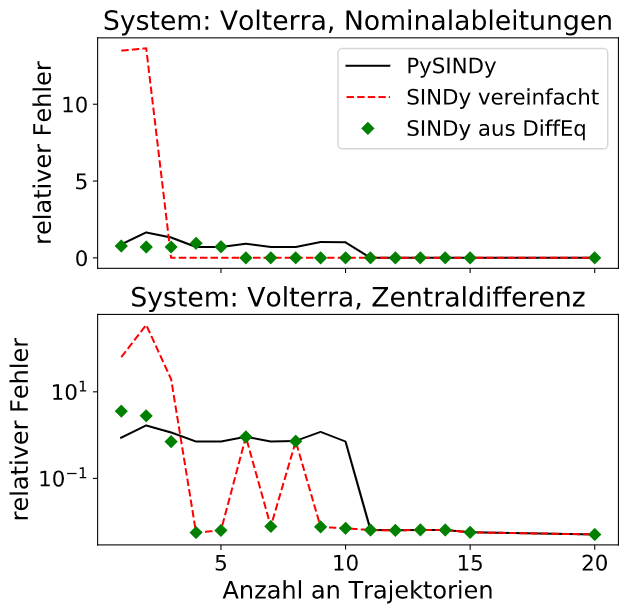
\includegraphics[width=75mm]{images/errors_volterra_no_tr_variation2.png}
	\caption{relativer Fehler der identifizierten Parameter in Abhängigkeit der Anzahl der gleichzeitig verwendeten Trajektorien.}
	\label{fig:errors_no_tr}
\end{figure}
\subsection{Identifikation von teilweise bekannten Systemen}
Rackauckas et al. \cite{Rackauckas2020} zeigen, wie man Wissen über bereits bekannte Teilsysteme in die Identifikation integrieren kann. Angenommen man möchte das Lotka-Volterra-System \eqref{eq:volterra} identifizieren und kennt bereits die linearen Terme und ihre Koeffizienten. Dann lässt sich das System darstellen als
\begin{equation}
	\begin{aligned}
		\dot{x} &= \alpha x + U_1(x,y)\\
		\dot{y} &= \gamma y + U_2(x,y),
	\end{aligned}
\end{equation}
mit den unbekannten nichtlinearen Termen $U_1(x,y)$ und $U_2(x,y)$. Da die Zustandsableitungen als bekannt angenommen werden (durch Messung oder Zentraldifferenz aus den Zuständen ermittelt), können die unbekannten Terme auf der rechten Seite isoliert werden:
\begin{equation}
	\begin{aligned}
		\dot{x} - \alpha x &= U_1(x,y)\\
		\dot{y} - \gamma y &= U_2(x,y).
	\end{aligned}
\end{equation}
Somit kann die angepasste linke Seite der Differentialgleichung folgendermaßen konstruiert werden:
\begin{equation}
\dot{X} = \begin{bmatrix} 
		\dot{x}(t_1)-\alpha x(t_1) & \dot{y}(t_1)-\gamma y(t_1) \\
		\dot{x}(t_2)-\alpha x(t_2) & \dot{y}(t_2)-\gamma y(t_2) \\
		\vdots 		   & \vdots 	 \\
		\dot{x}(t_m)-\alpha x(t_m) & \dot{y}(t_m)-\gamma y(t_m) \\
	\end{bmatrix}  \in \mathbb{R}^{m\times 2}.
\end{equation}
Von hier aus kann der Algorithmus wie bekannt weiterlaufen. 

Eine Voraussetzung für diese Methode ist, dass sich bekannte und unbekannte Teilsysteme voneinander isolieren lassen. Dies ist der Fall, wenn eine bekannte Funktion $K(\boldsymbol{x})\in\mathbb{R}^{n}$ und eine unbekannte Funktion $U(\boldsymbol{x})\in\mathbb{R}^{n}$ existieren, sodass die Umformung
\begin{equation}
 K(\boldsymbol{x}) \circ \dot{\boldsymbol{x}} = U(\boldsymbol{x})
\end{equation} 
möglich ist. Ist dies nicht der Fall, z.B. für
\begin{equation}
\dot{\boldsymbol{x}} = K_1(\boldsymbol{x})\cdot U_1(\boldsymbol{x}) + K_2(\boldsymbol{x})\cdot U_2(\boldsymbol{x}),
\end{equation}
dann kann das Wissen über das bekannte Teilsystem nur in die Gestaltung der Bibliothek einfließen, nicht jedoch die Identifikation wie beschrieben von Anfang an vereinfachen.
Dieses Problem wird in Abschnitt \ref{sec:aufbauderbibo} noch einmal aufgegriffen.








